\section{Numerical experiments}\label{sec:numerical_experiments}

In this section, we report numerical experiments conducted with the Julia implementation of our algorithm, named TRAULLS\footnote{Trust Region AUgmented nonLinear Least-squares Solver} on a Mac mini with an M4 processor and 24 GB of RAM. Our solver is open-source and can be downloaded from \url{https://github.com/UncertainLab/Traulls.jl}. All the benchmarks we present here are also accessible in the \texttt{benchmark} folder of the linked GitHub repository.
The tests were carried out on a set of 49 constrained NLS from collections~\cite{hockschittkowski:1980, schittkowski:1987, lucksanvlcek:1999} and problems 2 and 3 referenced in~\cite{biegler-etal2000}. For problems with variable dimensions, we set the number of variables to $n \in \{100, 500, 1000\}$. Thus, we have a total of 79 problem instances ranging from 2 to 1000 variables, with up to 2500 residuals and 1000 constraints. Problems with inequality constraints were converted to the form~\eqref{pb:cnls} by adding slack variables. For our tests, we set the criticality tolerance to $\omega_* = 10^{-5}$, the feasibility tolerance to $\eta_* = 10^{-6}$, the maximum number of outer iterations to 500 and the maximum number of iterations to 1000. We leave the other parameters of the algorithm at the values given at the end of Section~\ref{sec:algorithm}. We present our results with performance profiles of type~\citet{dolanmore:2002} produced with the \texttt{BenchmarkProfiles.jl} package~\cite{benchmark-profiles-julia}.

\subsection{Comparison of Hessian approximations}

Our first set of experiments compares the behavior and performance of our algorithm depending on the Hessian approximation used during the inner minimization. We compared the GN approximation~\eqref{eq:hessian_gn_approx} against structured approximations of the form~\eqref{eq:hessian_full_approx}. Based on the structured secant equation~\eqref{eq:structured_secant_eq}, we implemented the SR1 update we discussed and the BFGS update that one can derive similarly. Both structured approximations were used in their plain and hybrid variants with the switching rule~\eqref{eq:hybrid_update_strategy}.
We compared these five strategies against three metrics: computation time, number of outer iterations and number
of inner iterations. Results are indicated in Figure~\ref{fig:compare_hessians}. 
\begin{figure}[htbp]
	\centering
	\begin{subfigure}[b]{0.32\textwidth}
		\centering
		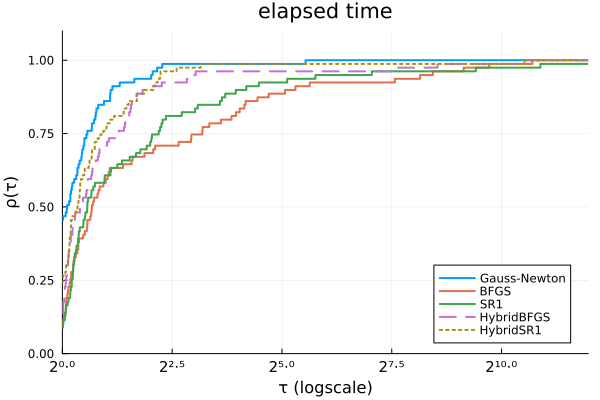
\includegraphics[width=\textwidth]{figures/traulls_all_hessians_time}
	\end{subfigure}
	\hfill
	\begin{subfigure}[b]{0.32\textwidth}
		\centering
		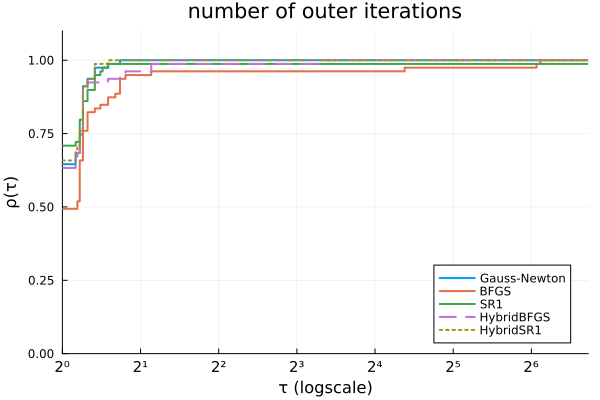
\includegraphics[width=\textwidth]{figures/traulls_all_hessians_outer}
	\end{subfigure}
	\hfill
	\begin{subfigure}[b]{0.32\textwidth}
		\centering
		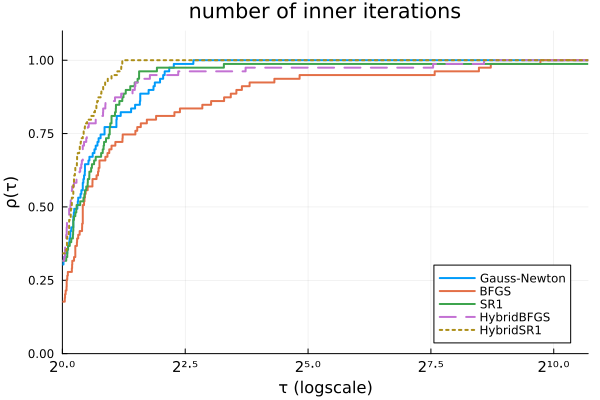
\includegraphics[width=\textwidth]{figures/traulls_all_hessians_inner}
	\end{subfigure}
	\caption{Performance profiles comparing five different Hessian approximations strategies with respect to computation time (left), number of outer iterations (center),
		and number of inner iterations (right).}
	\label{fig:compare_hessians}
\end{figure}
All five variants successfully solved all but one problem: the plain SR1 variant reaches the maximum number of iterations on the HS373 problem.
In terms of computation time, the GN approximation is the fastest: since it requires no	additional storage or update computation, it is the cheapest per iteration as our method mainly involves matrix-vector products. The GN approximation especially dominates on problems having sparse jacobians and small residuals at the solution, since the second order terms are still stored as a dense matrix. When measured by the number of inner iterations, the hybrid variants prove more efficient than their plain counterparts for both formulas. These observations are consistent with the discussion about the hybrid switching rule~\eqref{eq:hybrid_update_strategy} which -- as in the unconstrained case -- correctly identifies situations where the Gauss--Newton approximation must be corrected and activates the structured quasi-Newton correction accordingly. All approximation approaches are closer in terms of outer iterations, with plain BFGS a little bit behind, but overall, the Hybrid SR1 appears to be the most robust. To confirm these observations, we have focused our attention to a comparison of GN with Hybrid approximations, the latter appearing to be the most efficient. Profiles in Figure~\ref{fig:gn_vs_hybrid} compare the 3 approaches against the number of residual and gradient evaluations. The latter are similar to the inner iterations profile previously shown, as we evaluate the residuals one time per inner iteration and evaluate the gradient at every accepted step.
Nevertheless, Hybrid-SR1 exhibits the best efficiency and robustness. This also seems to indicate that the SR1 approximation is adequate with the negative curvature handling in the trust region setting. 
\begin{figure}[htbp]
	\centering
	\begin{subfigure}[b]{0.45\textwidth}
		\centering
		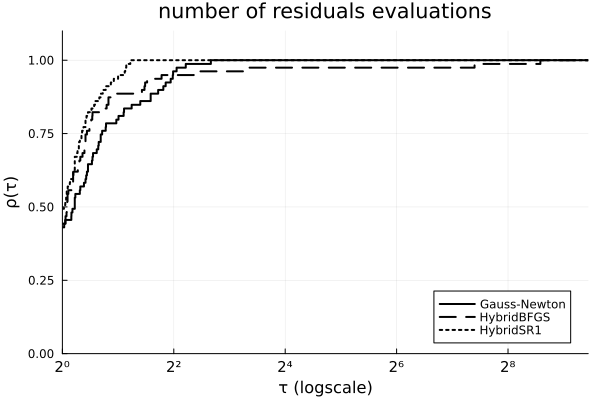
\includegraphics[width=\textwidth]{figures/gn_vs_hybrid_reseval_profile}
	\end{subfigure}
	\hfill
	\begin{subfigure}[b]{0.45\textwidth}
		\centering
		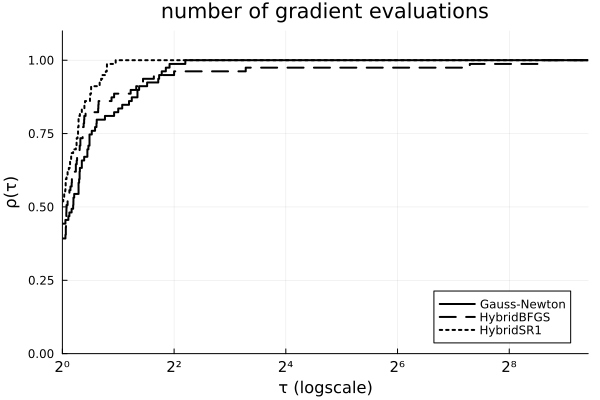
\includegraphics[width=\textwidth]{figures/gn_vs_hybrid_gradeval_profile}
	\end{subfigure}
	\caption{Performance profiles comparing the Gauss-Newton approximation against hybrid approaches with respect to the number of residual evaluations (left),
		and gradient evaluations (right).}
	\label{fig:gn_vs_hybrid}
\end{figure}
Based on these results, we retain the Hybrid SR1 variant as the best overall strategy for
TRAULLS, and use it in the comparisons that follow.

\subsection{Comparison with IPOPT and Percival}

We now compare TRAULLS (with the Hybrid SR1 approximation) against solvers IPOPT~\cite{wachterbiegler:2006} and Percival~\cite{arreckx-etal:2016}. The latter is also an augmented Lagrangian algorithm and has a native Julia implementation and uses a Julia version of the TRON~\cite{linmore:1999a} algorithm -- part of the \texttt{JSOSolvers.jl} package~\cite{migot-etal:2026} -- for the inner minimization. To benefit from the benchmarking facilities provided by the JuliaSmoothOptimizers (JSO)\footnote{https://jso.dev/} ecosystem, we used the wrapper \texttt{NLPModelsIpopt.jl}~\cite{nlp-models-ipopt-julia}. This allows us to run both solvers on our test set of problems -- all models being encoded in \texttt{NLSProblems.jl}~\cite{nls-problems-julia} -- and export the benchmark metrics using \texttt{SolverBenchmark.jl}~\cite{solver-benchmark-julia}.  To make the comparison with IPOPT relevant, we have set the parameters \texttt{nlp\_scaling\_method} = \texttt{none}, \texttt{dual\_inf\_tol} = \texttt{Inf}, \texttt{constr\_viol\_tol} = \texttt{Inf}, \texttt{compl\_inf\_tol }= \texttt{Inf}, \texttt{acceptable\_iter} = \texttt{0} and the maximum number of iterations to 1000. For Percival, since it also follows Algorithm~\ref{algo:traulls}, we have set its tolerances and parameters to the same value as ours.
For these tests, we compare the three solvers against the CPU time, the number of residual evaluations and the number of gradient evaluations. The results are presented in Figure~\ref{fig:perf_solvers}. During our experiments, IPOPT reached the maximum number of iterations on problem HS27 and returned the \texttt{unknown} internal message on problem HS70. Percival reached the maximum of iterations on the two instances of problem 5.11 from~\cite{lucksanvlcek:1999} having $n=500$ and $n=1000$.
\begin{figure}[htbp]
	\centering
	\begin{subfigure}[b]{0.32\textwidth}
		\centering
		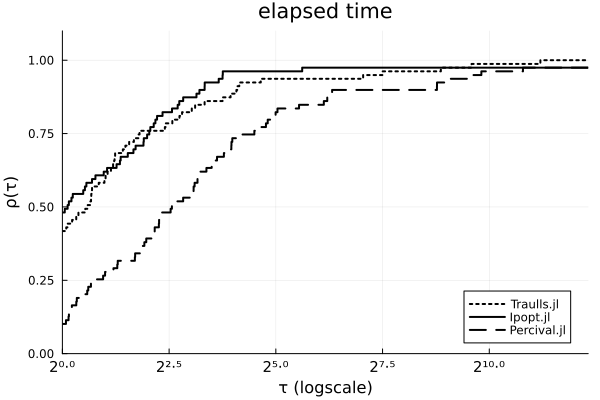
\includegraphics[width=\textwidth]{figures/traulls_vs_others_time_profile}
	\end{subfigure}
	\hfill
	\begin{subfigure}[b]{0.32\textwidth}
		\centering
		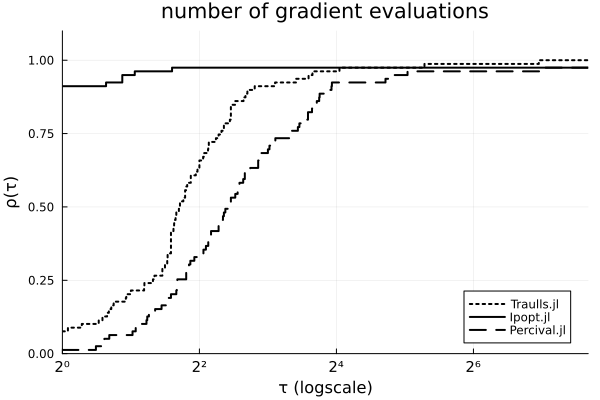
\includegraphics[width=\textwidth]{figures/traulls_vs_others_gradeval_profile}
	\end{subfigure}
	\hfill
	\begin{subfigure}[b]{0.32\textwidth}
		\centering
		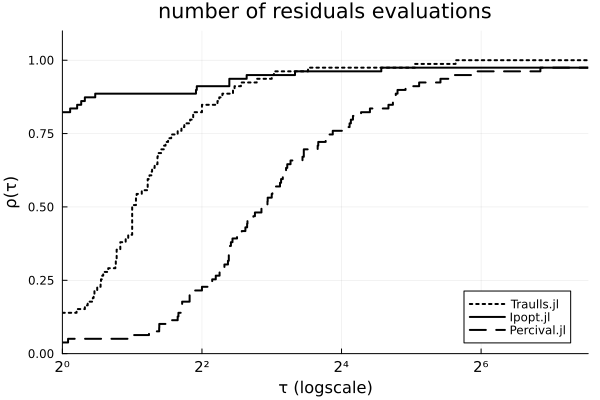
\includegraphics[width=\textwidth]{figures/traulls_vs_others_reseval_profile}
	\end{subfigure}
	\caption{Performance profiles comparing TRAULLS (Hybrid SR1), IPOPT, and Percival
		on the test set, with respect to computation time (left), residual evaluations (center),
		and gradient evaluations (right).}
	\label{fig:perf_solvers}
\end{figure}

In terms of computation time, TRAULLS and IPOPT achieve comparable performance, with
IPOPT holding a modest advantage on the fastest problems but the gap narrowing as
problem difficulty increases. Percival is consistently slower than both solvers across the
test set. Regarding the function-evaluation metrics, IPOPT dominates: its interior-point
strategy, which exploits second-order information through exact Hessians, requires
significantly fewer residual and gradient evaluations to reach convergence. TRAULLS, which
relies on a structured quasi-Newton approximation and therefore does not require exact
second derivatives, performs comparably to Percival on these metrics and outperforms it on
a majority of problems.
Across all three metrics, IPOPT is a clear winner, in spite of the two failures. However, our method is a close second in computation time and achieves similar robustness with regard to the number of residual evaluations. The clear advantage of TRAULLS over Percival shows that within the same algorithmic framework, exploiting the least-squares structures leads to better performance.